%%%%%%%%%%%%%%%%%%%%%%%%%%%%%%%%%%%%%%%%%%%%%%%%%%%%%%%%%%%%%%%%%%%%%%%%%%%%%%%%%%%%%%%%%%%%%%%%%%%%%%%%%%%%%%%%%%%%%%%%%%%%%%%%%%%%%%%%%%%%%%%%%%%%%%%%%%%%%%%%%%%%%%%
%%%%%%%%%%%%%%%%%%%%%%%%%%%%%%%%%%%%%%%%%%%%%%%%%%%%%%%%%%%%%%%%%%%%%%%%%%%%%%%%%%%%%%%%%%%%%%%%%%%%%%%%%%%%%%%%%%%%%%%%%%%%%%%%%%%%%%%%%%%%%%%%%%%%%%%%%%%%%%%%%%%%%%%
%%% Modèle pour la 1ère de couverture des thèses préparées à l'Université Paris-Saclay, basé sur le modèle produit par Guillaume BRIGOT / Template for back cover of thesis made at Université Paris-Saclay, based on the template made by Guillaume BRIGOT
%%% Mis à jour par Aurélien ARNOUX (École polytechnique)/ Updated by Aurélien ARNOUX (École polytechnique)
%%% Les instructions concernant chaque donnée à remplir sont données en bloc de commentaire / Rules to fill this file are given in comment blocks
%%% ATTENTION Ces informations doivent tenir sur une seule page une fois compilées / WARNING These informations must contain in no more than one page once compiled
%%%%%%%%%%%%%%%%%%%%%%%%%%%%%%%%%%%%%%%%%%%%%%%%%%%%%%%%%%%%%%%%%%%%%%%%%%%%%%%%%%%%%%%%%%%%%%%%%%%%%%%%%%%%%%%%%%%%%%%%%%%%%%%%%%%%%%%%%%%%%%%%%%%%%%%%%%%%%%%%%%%%%%%
%%% Version du 23 mai 2019 (Merci à Thibault CHEVALÉRIAS (CEA) pour ses suggestions et corrections)
%%%%%%%%%%%%%%%%%%%%%%%%%%%%%%%%%%%%%%%%%%%%%%%%%%%%%%%%%%%%%%%%%%%%%%%%%%%%%%%%%%%%%%%%%%%%%%%%%%%%%%%%%%%%%%%%%%%%%%%%%%%%%%%%%%%%%%%%%%%%%%%%%%%%%%%%%%%%%%%%%%%%%%%


\label{form_first}

%%% Formulaire / Form
%%% Remplacer les paramètres des \newcommand par les informations demandées / Replace \newcommand parameters by asked informations
%%%


\newcommand{\NNT}{20XXSACLXXXX} 															%% Numéro National de Thèse (donnée par la bibliothèque à la suite du 1er dépôt)/ National Thesis Number (given by the Library after the first deposit)

\newcommand{\ecodoctitle}{École Doctorale MSTII - Mathématiques, Sciences et
technologies de l'information, Informatique} 													%% Nom de l'ED. Voir site de l'Université Paris-Saclay / Full name of Doctoral School. See Université Paris-Saclay website
\newcommand{\ecodocacro}{ed-mstii}																%% Sigle de l'ED. Voir site de l'Université Paris-Saclay / Acronym of the Doctoral School. See Université Paris-Saclay website
\newcommand{\ecodocnum}{217} 																%% Numéro de l'école doctorale / Doctoral School number
\newcommand{\PhDspeciality}{Informatique} 										%% Spécialité de doctorat / Speciality 
\newcommand{\PhDworkingplace}{Maison de la Simulation} 										%% Établissement de préparation / PhD working place : l'Université Paris-Sud, l'Université de Versailles-Saint-Quentin-en-Yvelines, l'Université d'Evry-Val-d'Essonne, l'Institut des sciences et industries du vivant et de l'environnement (AgroParisTech), CentraleSupélec,l'Ecole normale supérieure de Cachan, l'Ecole Polytechnique, l'Ecole nationale supérieure de techniques avancées, l'Ecole nationale de la statistique et de l’administration économique, HEC Paris, l'Institut d'optique théorique et appliquée, Télécom ParisTech, Télécom SudParis   
\newcommand{\defenseplace}{Gif-Sur-Yvette} 											%% Ville de soutenance / Place of defense
\newcommand{\defensedate}{Date} 															%% Date de soutenance / Date of defense

%%% Établissement / Institution
%%% Si la thèse a été produite dans le cadre d'une co-tutelle, commenter la partie "Pas de co-tutelle" et décommenter la partie "Co-tutelle" / If the thesis has been prepared in guardianship, comment the part "Pas de co-tutelle" and uncomment the part "Co-tutelle"

	%%%%%%%%%%%%%%%%%%%%%%%%%
	%%% Pas de co-tutelle %%%
	%%%%%%%%%%%%%%%%%%%%%%%%%

\newcommand{\logoEtt}{blank}																%% NE PAS MODIFIER / DO NOT MODIFY
\newcommand{\vpostt}{0.1} 																	%% NE PAS MODIFIER / DO NOT MODIFY
\newcommand{\hpostt}{6}																		%% NE PAS MODIFIER / DO NOT MODIFY
\newcommand{\logoEt}{etab} 																	%% Logo de l'établissement de soutenance. Indiquer le sigle / Institution logo. Indicate the acronym : AGRO, CENTSUP, ENS, ENSAE, ENSTA, HEC, IOGS, TPT, TSP, UEVE, UPSUD, UVSQ, X 
\newcommand{\vpos}{0.1}																		%% À modifier au besoin pour aligner le logo verticalement / If needed, modify to align logo vertilcally
\newcommand{\hpos}{11}																		%% À modifier au besoin pour aligner le logo horizontalement / If needed, modify to align logo horizontaly

		%%%%%%%%%%%%%%%%%%
		%%% Co-tutelle %%%
		%%%%%%%%%%%%%%%%%%

%\newcommand{\logoEt}{etab} 																%% Logo de l'université partenaire. Placer le fichier .png dans le répertoire '/media/etab' et indiquer le nom du fichier sans l'extension / Logo of partner university. Place the .png file in the directory '/media/etab' and point the file name without the extension
%\newcommand{\vpos}{0.1}																	%% À modifier au besoin pour aligner les logos verticalement / If needed, modify to align logos vertilcally
%\newcommand{\hpos}{11}																		%% À modifier au besoin pour aligner les logos horizontalement / If needed, modify to align logos horizontaly
%\newcommand{\logoEtt}{etab2}  																%% Logo de l'établissement de soutenance. Le nom du fichier correspond au sigle de l'établissement /  Institution logo. Filename correspond to institution acronym : AGRO, CENTSUP, ENS, ENSAE, ENSTA, HEC, IOGS, TPT, TSP, UEVE, UPSUD, UVSQ, X 
%\newcommand{\vpostt}{0.1} 																	%% À modifier au besoin pour aligner les logos verticalement / If needed, modify to align logos vertilcally
%\newcommand{\hpostt}{6}																	%% À modifier au besoin pour aligner les logos horizontalement / If needed, modify to align logos horizontaly


%%% JURY

% Lors du premier dépôt de la thèse le nom du président n’est pas connu, le choix du président se fait par les membres du Jury juste avant la soutenance. La précision est apportée sur la couverture lors du second dépôt / Choice of the jury's president is made during the defense. Thus, it must be specified only for the second file deposition in ADUM.
% Tous les membres du juty listés doivent avoir été présents lors de la soutenance / All the jury members listed here must have been present during the defense.

%%% Membre n°1 (Président) / Member n°1 (President)
\newcommand{\jurynameA}{Prénom Nom}
\newcommand{\juryadressA}{Statut, Établissement (Unité de recherche)}
\newcommand{\juryroleA}{Président}

%%% Membre n°2 (Rapporteur) / Member n°2 (Reviewer)
\newcommand{\jurynameB}{Prénom Nom}
\newcommand{\juryadressB}{Statut, Établissement (Unité de recherche)}
\newcommand{\juryroleB}{Rapporteur}

%%% Membre n°3 (Rapporteur) / Member n°3 (Reviewer)
\newcommand{\jurynameC}{Prénom Nom}
\newcommand{\juryadressC}{Statut, Établissement (Unité de recherche)}
\newcommand{\juryroleC}{Rapporteur}

%%% Membre n°4 (Examinateur) / Member n°4 (Examiner)
\newcommand{\jurynameD}{Prénom Nom}
\newcommand{\juryadressD}{Statut, Établissement (Unité de recherche)}
\newcommand{\juryroleD}{Examinateur}

%%% Membre n°5 (Directeur de thèse) / Member n°5 (Thesis supervisor)
\newcommand{\jurynameE}{Bruno RAFFIN}
\newcommand{\juryadressE}{Statut, Établissement (Unité de recherche)}
\newcommand{\juryroleE}{Directeur de thèse}

%%% Membre n°6 (Co-directeur de thèse) / Member n°6 (Thesis co-supervisor)
\newcommand{\jurynameF}{Julien BIGOT}
\newcommand{\juryadressF}{Statut, Établissement (Unité de recherche)}
\newcommand{\juryroleF}{Co-encadrant de thèse}

%%% Membre n°7 (Invité) / Member n°7 (Guest)
\newcommand{\jurynameG}{Prénom Nom}
\newcommand{\juryadressG}{Statut, Établissement (Unité de recherche)}
\newcommand{\juryroleG}{Invité}

%%% Membre n°8 (Invité) / Member n°8 (Guest)
\newcommand{\jurynameH}{Prénom Nom}
\newcommand{\juryadressH}{Statut, Établissement (Unité de recherche)}
\newcommand{\juryroleH}{Invité}

%% Il est possible d'ajouter des membres supplémentaires selon le même modèle / More jury members can be added according to the same model

\label{layout_first}
%%% Mise en page / Page layout      
%%% NE RIEN MODIFIER EXCEPTÉ LA PARTIE CONCERNANT LE JURY (voir \label{jury}) SI BESOIN / DO NOT MODIFY EXCEPT SECTION CONCERNING JURY (see \label{jury}) IF NEEDED
%%%%%%%%%%%%%%%%%%%%%%%%%%%%%%%%%%%%%%%%%%%%%%%%%%%%%%%%%%%%%%%%%%%%%%%%%%%%%%%%%%%%%%%%%%%%%%%%%%%%%%%%%%%%%%%%%%%%%%%%%%%%%%%%%%%%%%%%%%%%%%%%%%%%%%%%%%%%%%%%%%%%%%%
%%%%%%%%%%%%%%%%%%%%%%%%%%%%%%%%%%%%%%%%%%%%%%%%%%%%%%%%%%%%%%%%%%%%%%%%%%%%%%%%%%%%%%%%%%%%%%%%%%%%%%%%%%%%%%%%%%%%%%%%%%%%%%%%%%%%%%%%%%%%%%%%%%%%%%%%%%%%%%%%%%%%%%%




\thispagestyle{empty}

%% Texte
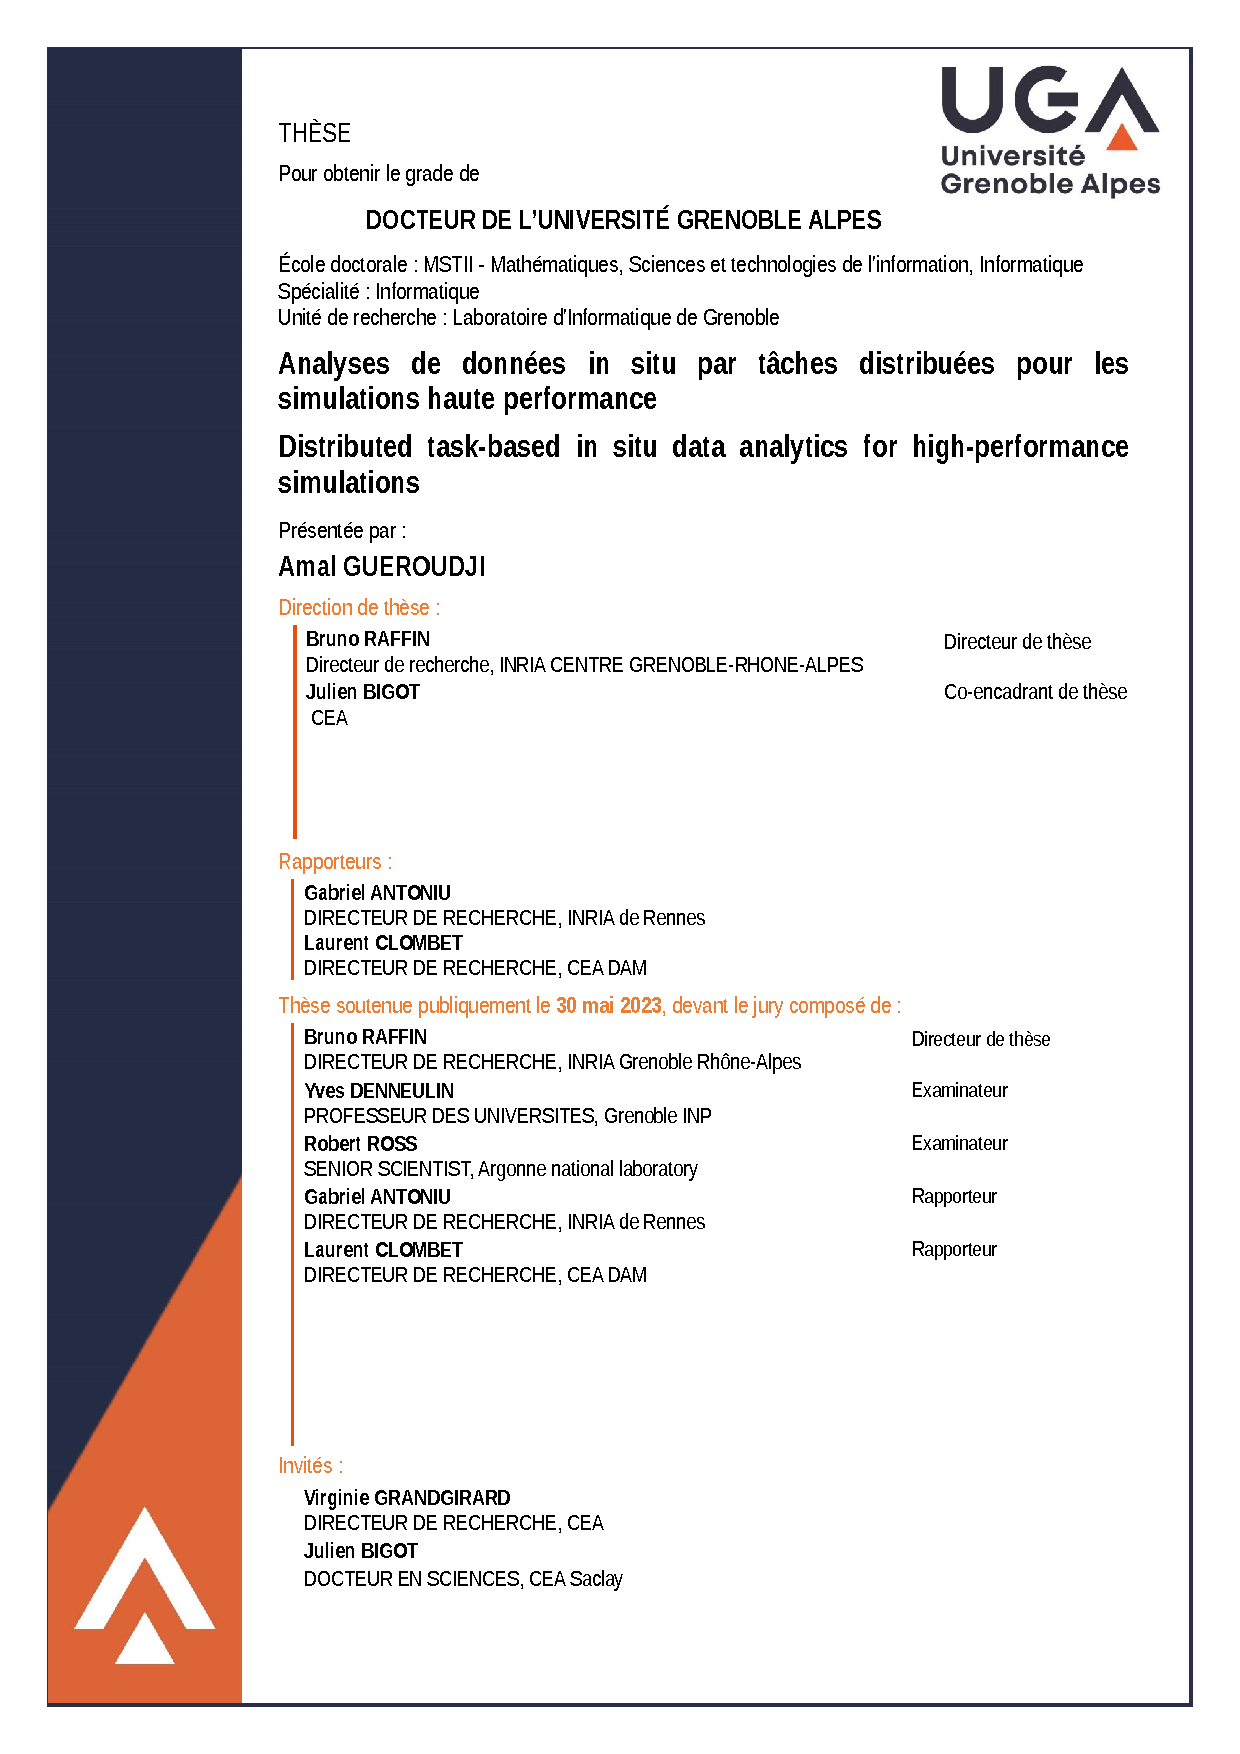
\includepdf[pages=-]{layout/couverture.pdf}

%\afterpage{\blankpage}